% Volume of the unit ball V_n = pi^(n/2)/Gamma(n/2+1), n = 0..20. Generated by a short script.
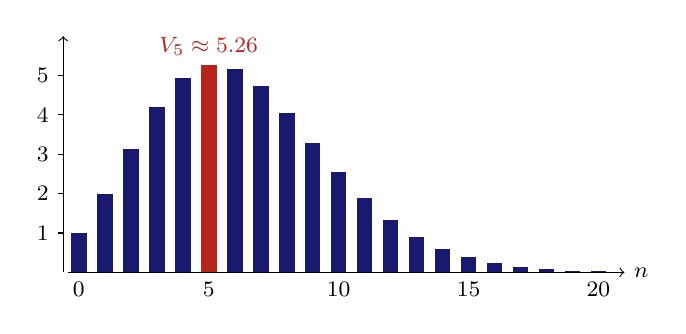
\begin{tikzpicture}[every node/.style={font=\footnotesize}]
\fill[MidnightBlue] (-0.100,0) rectangle (0.100,0.500);
\fill[MidnightBlue] (0.230,0) rectangle (0.430,1.000);
\fill[MidnightBlue] (0.560,0) rectangle (0.760,1.571);
\fill[MidnightBlue] (0.890,0) rectangle (1.090,2.094);
\fill[MidnightBlue] (1.220,0) rectangle (1.420,2.467);
\fill[BrickRed] (1.550,0) rectangle (1.750,2.632);
\fill[MidnightBlue] (1.880,0) rectangle (2.080,2.584);
\fill[MidnightBlue] (2.210,0) rectangle (2.410,2.362);
\fill[MidnightBlue] (2.540,0) rectangle (2.740,2.029);
\fill[MidnightBlue] (2.870,0) rectangle (3.070,1.649);
\fill[MidnightBlue] (3.200,0) rectangle (3.400,1.275);
\fill[MidnightBlue] (3.530,0) rectangle (3.730,0.942);
\fill[MidnightBlue] (3.860,0) rectangle (4.060,0.668);
\fill[MidnightBlue] (4.190,0) rectangle (4.390,0.455);
\fill[MidnightBlue] (4.520,0) rectangle (4.720,0.300);
\fill[MidnightBlue] (4.850,0) rectangle (5.050,0.191);
\fill[MidnightBlue] (5.180,0) rectangle (5.380,0.118);
\fill[MidnightBlue] (5.510,0) rectangle (5.710,0.070);
\fill[MidnightBlue] (5.840,0) rectangle (6.040,0.041);
\fill[MidnightBlue] (6.170,0) rectangle (6.370,0.023);
\fill[MidnightBlue] (6.500,0) rectangle (6.700,0.013);
\draw[->] (-0.132,0)--(6.930,0) node[right] {$n$};
\draw[->] (-0.198,0)--(-0.198,3.000);
\node[below] at (0.000,0) {$0$};
\node[below] at (1.650,0) {$5$};
\node[below] at (3.300,0) {$10$};
\node[below] at (4.950,0) {$15$};
\node[below] at (6.600,0) {$20$};
\draw (-0.198,0.500)--(-0.258,0.500) node[left] {$1$};
\draw (-0.198,1.000)--(-0.258,1.000) node[left] {$2$};
\draw (-0.198,1.500)--(-0.258,1.500) node[left] {$3$};
\draw (-0.198,2.000)--(-0.258,2.000) node[left] {$4$};
\draw (-0.198,2.500)--(-0.258,2.500) node[left] {$5$};
\node[BrickRed,above] at (1.650,2.635) {$V_5\approx5.26$};
\end{tikzpicture}
